% Technical report of the Java implementation of Stage 1.
% Build from java/stage1/docs/report/:
%   uv run --with matplotlib python charts.py     (figures/*.pdf, from benchmarks/results/)
%   pdflatex report.tex && pdflatex report.tex     (twice, for the table of contents)
\documentclass[11pt,a4paper]{article}

\usepackage[utf8]{inputenc}
\usepackage[T1]{fontenc}
\usepackage{lmodern}
\usepackage{microtype}
\usepackage[margin=2.4cm,headheight=14pt]{geometry}
\usepackage{graphicx}
\usepackage{booktabs}
\usepackage{tabularx}
\usepackage{longtable}
\usepackage{array}
\usepackage{enumitem}
\usepackage{float}
\usepackage{xcolor}
\usepackage{listings}
\usepackage{tikz}
\usetikzlibrary{positioning,arrows.meta,fit,calc}
\usepackage{fancyhdr}
\usepackage{titlesec}
\usepackage[hidelinks]{hyperref}

\definecolor{accent}{HTML}{2a78d6}
\definecolor{ink}{HTML}{0b0b0b}
\definecolor{muted}{HTML}{52514e}
\definecolor{codebg}{HTML}{f6f6f4}
\definecolor{rule}{HTML}{d8d7d2}
\definecolor{notebg}{HTML}{eef4fc}

\hypersetup{colorlinks=true,linkcolor=accent,urlcolor=accent,citecolor=accent}

\titleformat{\section}{\Large\bfseries\color{ink}}{\thesection.}{0.6em}{}
\titleformat{\subsection}{\large\bfseries\color{ink}}{\thesubsection}{0.6em}{}
\titleformat{\subsubsection}{\normalsize\bfseries\color{ink}}{\thesubsubsection}{0.6em}{}
\titlespacing*{\section}{0pt}{1.6em}{0.7em}
\titlespacing*{\subsection}{0pt}{1.2em}{0.5em}

\pagestyle{fancy}
\fancyhf{}
\fancyhead[L]{\small\color{muted}Stage 1 $\cdot$ Data layer $\cdot$ Java implementation}
\fancyhead[R]{\small\color{muted}Big Data $\cdot$ ULPGC}
\fancyfoot[C]{\small\thepage}
\renewcommand{\headrulewidth}{0.4pt}

\setlist{itemsep=2pt,topsep=4pt}
\setlength{\parskip}{0.45em}
\setlength{\parindent}{0pt}
\setlength{\emergencystretch}{3em}   % long \texttt names: stretch spaces rather than overflow
\renewcommand{\arraystretch}{1.25}

\lstdefinestyle{java}{
  language=Java, basicstyle=\ttfamily\footnotesize, backgroundcolor=\color{codebg},
  keywordstyle=\color{accent}\bfseries, commentstyle=\color{muted}\itshape,
  stringstyle=\color{ink}, frame=single, rulecolor=\color{rule}, framesep=4pt,
  xleftmargin=6pt, xrightmargin=6pt, breaklines=true, columns=fullflexible,
  keepspaces=true, showstringspaces=false, aboveskip=8pt, belowskip=8pt}
\lstdefinestyle{shell}{
  language={}, basicstyle=\ttfamily\footnotesize, backgroundcolor=\color{codebg}, frame=single,
  rulecolor=\color{rule}, framesep=4pt, xleftmargin=6pt, xrightmargin=6pt,
  breaklines=true, columns=fullflexible, keepspaces=true, showstringspaces=false,
  aboveskip=8pt, belowskip=8pt, literate={í}{{\'i}}1 {ó}{{\'o}}1 {á}{{\'a}}1}
\lstset{style=java}

\newcolumntype{Y}{>{\raggedright\arraybackslash}X}
\newcommand{\code}[1]{\texttt{#1}}
\newcommand{\us}{\,$\mu$s}
\newenvironment{note}{\par\smallskip\noindent
\begin{tikzpicture}\node[fill=notebg,draw=accent!40,rounded corners=2pt,inner sep=7pt,text width=\dimexpr\linewidth-14pt\relax]\bgroup\small}{\egroup;\end{tikzpicture}\par\smallskip}

% One class card in the code walkthrough: \cls{Name}{kind}{description}
\newcommand{\cls}[2]{\par\medskip\noindent{\large\bfseries\code{#1}}\hspace{0.6em}{\small\color{muted}#2}\par\nopagebreak\smallskip}
\newcommand{\why}[1]{\par\noindent\textit{Design rationale.} #1\par}

\begin{document}

% ---------------------------------------------------------------- title page
\begin{titlepage}
\thispagestyle{empty}
\vspace*{2.5cm}
{\color{accent}\rule{\linewidth}{1.2pt}}\\[0.8cm]
{\Huge\bfseries Search Engine Project\par}
\vspace{0.4cm}
{\LARGE Stage 1: Building the Data Layer\par}
\vspace{0.6cm}
{\Large\color{muted} Java implementation --- technical report\par}
\vspace{0.6cm}
{\color{accent}\rule{\linewidth}{1.2pt}}
\vspace{2cm}

\begin{tabular}{@{}>{\bfseries}p{3.4cm}p{10.5cm}@{}}
Course & Big Data $\cdot$ Grado en Ciencia e Ingeniería de Datos $\cdot$ Universidad de Las Palmas de Gran Canaria \\
Academic year & 2026/2027 \\
Group name & BigData-Ulpgc \\
Members & Daniel Rodríguez Alonso --- Java implementation, author of this report \\
 & Daniel Perdomo Medina --- Python implementation \\
 & Carlos Falcón Brito --- C++ implementation \\
Repository & \url{https://github.com/BigData-Ulpgc/stage_1}, branch \code{java}, folder \code{java/stage1/} \\
Status & Complete pipeline, offline mode with the sample dataset, 12 benchmark experiments, 357 tests passing \\
Date & 4 October 2026 \\
\end{tabular}

\vfill
\begin{note}
\textbf{Quick check for instructors.} From \code{java/stage1/}, with JDK~17+ and Maven, and no network:
\code{mvn package}, then \code{java -cp "\$CP" es.ulpgc.bigdata.Main pipeline 30 -{}-offline} and
\code{java -cp "\$CP" es.ulpgc.bigdata.Main search whale island}. Section~\ref{sec:quick} gives the
exact commands and the expected output.
\end{note}
\end{titlepage}

% ---------------------------------------------------------------- abstract + toc
\section*{Abstract}
This report describes the Java implementation of Stage~1 of the group's search engine over
Project Gutenberg books. Stage~1 builds the \emph{data layer}: a pipeline that downloads books,
splits each one into header and body, stores them in a datalake, extracts their metadata into a
SQLite datamart and builds an inverted index that answers Boolean AND queries. A control layer
records the progress so an interrupted run resumes without losing or repeating books.

The implementation offers three datalake layouts (\code{book}, \code{range}, \code{time}) and three
persistent inverted-index structures (\code{monolithic} JSON, \code{hierarchical} folders,
\code{mongo}), selectable through configuration without touching code. It follows the group's
common contract (\code{shared/SPEC.md}), so its outputs match the Python and C++ implementations. A
15-book sample dataset lets the whole pipeline run offline in about one second. The 12 benchmark
experiments, run on the 200 real books of the dataset, show that the \code{monolithic} index is the
fastest to build and query but is the only one whose update cost and memory grow with the index;
that \code{hierarchical} wastes about 73 times its data size in file-system blocks; and that the
\code{time} datalake pays for its arrival-order layout with lookups about 29 times slower than
\code{book}.

\tableofcontents
\newpage

% ================================================================ 1
\section{Introduction and objectives}

\subsection{Goal of Stage 1}
The final goal of the course project is a search engine over books from Project Gutenberg. Stage~1
does not yet aim at ranking or a user interface. It builds the data layer underneath: books must be
downloaded, stored, described and indexed \emph{correctly}, in a way that \emph{recovers from
failures}, and \emph{measurably}, so that several ways of organising the data can be compared.

\begin{table}[H]
\centering\small
\begin{tabularx}{\linewidth}{@{}l Y l@{}}
\toprule
Layer & What it does & Java package \\
\midrule
Ingestion & Downloads the text from Gutenberg and splits it into header (title, author\ldots) and body (the book itself); the licence footer is discarded. & \code{crawler} \\
Datalake & Stores header and body as files, in one of three layouts: \code{book}, \code{range} or \code{time}. & \code{datalake} \\
Datamarts & Processed data ready to query: metadata in SQLite, and the inverted index (term $\rightarrow$ books) in three variants. & \code{datamart.*} \\
Query & AND search: the books that contain every term of the query. & \code{query} \\
Control & Files that remember which books are downloaded and indexed, so work is never repeated or lost. & \code{control} \\
Configuration & One place for paths, timeouts and active structures; factories that map names to implementations. & \code{config} \\
Benchmarks & Measure and compare the structures with a common methodology, writing CSV results. & \code{benchmark} \\
\bottomrule
\end{tabularx}
\caption{The layers of the system and where each lives in the Java code.}
\end{table}

\subsection{The group and the common contract}
The group implements the same data layer three times: in Java (this report), Python and C++. So
that the three can be compared, the group agreed on a common contract, \code{shared/SPEC.md}, which
fixes everything that must not differ between languages. Many design decisions in the Java code
follow directly from it.

\begin{table}[H]
\centering\small
\begin{tabularx}{\linewidth}{@{}l Y@{}}
\toprule
SPEC section & Rule \\
\midrule
1. Dataset & \code{book\_ids.txt} (ids to download, in order), \code{queries.txt} (benchmark queries), \code{stopwords.txt}. Empty lines and lines starting with \code{\#} are ignored. \\
2. Split & Markers \code{*** START OF THE/THIS PROJECT GUTENBERG EBOOK} and \code{*** END OF \ldots}. If either is missing, the book is discarded. Header = text before START (trimmed); body = from the end of the START line to END (trimmed); \code{\textbackslash r\textbackslash n} $\rightarrow$ \code{\textbackslash n}. \\
3. Datalake & \code{time}: \code{YYYYMMDD/HH/<ID>.body.txt}; \code{book}: \code{<ID>/body.txt}; \code{range}: \code{<START>-<END>/<ID>.body.txt}, with START $= \lfloor ID/1000\rfloor\cdot 1000$ in 5 digits. \\
4. Metadata & \code{title}, \code{author}, \code{release\_date}, \code{language} by multi-line regex, first match, first line only, trimmed; missing $\rightarrow$ NULL. SQLite table \code{books} with indexes on \code{author} and \code{title}. \\
5. Tokenizer & Character by character: A--Z $\rightarrow$ lowercase; a--z and 0--9 form tokens; anything else separates (accents and apostrophes included). Tokens shorter than 2 and stopwords are dropped. Each book contributes its \emph{set} of terms (no frequencies). \\
6. Index & \code{monolithic}: one JSON \code{\{"term":[ids]\}}; \code{hierarchical}: \code{inverted\_index/<LETTER>/<term>.txt}; \code{mongo}: collection \code{inverted\_index} with a unique index on \code{term}. Posting lists sorted, without duplicates. \\
7. Queries & The query goes through the same tokenizer; AND = intersection; ids sorted. \\
8. Control & \code{control/downloaded\_books.txt} and \code{indexed\_books.txt}; an id is appended only after its step succeeded. \\
9--10. Benchmarks & CSV \code{language,experiment,structure,} \code{dataset\_size,repetition,metric,value,unit}; 2 warm-ups + 5 measured runs; no network inside a measurement; the 200 real books, size N = the N lowest ids; reference term and posting counts. \\
\bottomrule
\end{tabularx}
\caption{Summary of the common contract, \code{shared/SPEC.md}.}
\end{table}

\subsection{Objectives and scope of this report}
The objectives of Stage~1, as set by the assignment, are to build a datalake for the raw books and
datamarts for structured, queryable data (metadata and inverted index); to coordinate them with a
minimal control layer that never duplicates or loses work; and to benchmark alternative datalake and
inverted-index structures, implemented in at least three programming languages over the same data.

This report covers the \textbf{Java} implementation of the group's project. It explains its
architecture, its design decisions and every class of its code, how to run and test it, and the
results of its benchmarks. The Python and C++ implementations follow the same contract and are
documented in their own folders of the repository.

The Java implementation delivers:
\begin{itemize}
  \item The complete pipeline: crawler, datalake, metadata datamart, inverted-index datamart, AND
        query and control layer, behind a small command-line interface (\code{Main}).
  \item All three datalake layouts and all three persistent index structures of the SPEC, plus an
        in-memory index used as a reference in tests. The active ones are chosen in
        \code{config.properties} or with \code{-D} options.
  \item An \textbf{offline mode} that runs the same pipeline on the 15 books of
        \code{sample\_dataset/}, so instructors can test everything without network.
  \item All 12 benchmark experiments of the SPEC, in its CSV format, with results committed in
        \code{benchmarks/results/real/} and \code{synthetic/}.
  \item 357 JUnit~5 tests at four levels (unit, contract, integration and end-to-end), including one
        that checks the output against the sample dataset's reference values.
\end{itemize}

% ================================================================ 2
\section{System architecture}

Figure~\ref{fig:components} follows one book through the system. Every storage box is an interface
with several interchangeable implementations.

\begin{figure}[H]
\centering
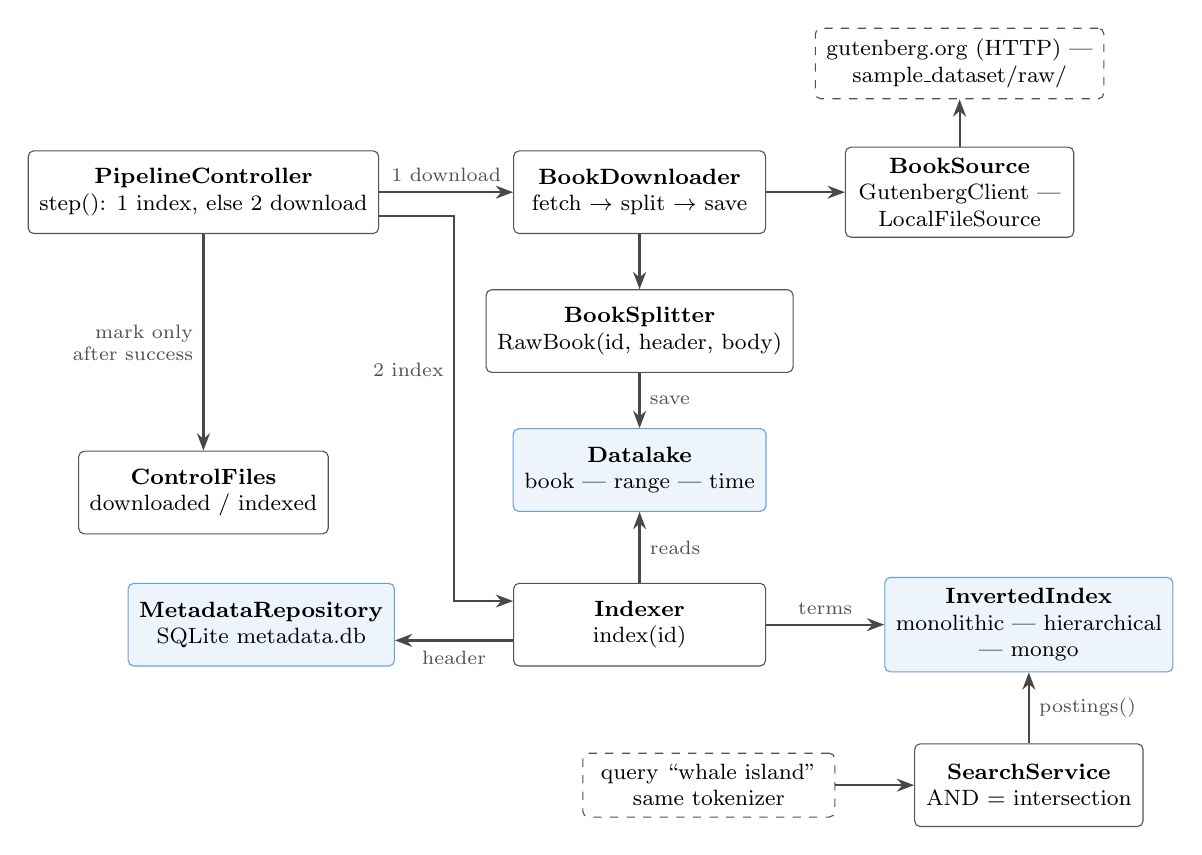
\begin{tikzpicture}[
  font=\footnotesize,
  box/.style={draw=ink!70,rounded corners=2pt,align=center,minimum height=1.05cm,inner sep=4pt,fill=white},
  store/.style={box,fill=notebg,draw=accent!70},
  ext/.style={box,dashed,draw=muted},
  arr/.style={-{Stealth[length=2.2mm]},thick,draw=ink!75},
  lbl/.style={font=\scriptsize,color=muted}]
  \node[box,minimum width=3.0cm] (pc) {\textbf{PipelineController}\\step(): 1 index, else 2 download};
  \node[box,right=1.7cm of pc,minimum width=3.2cm] (dl) {\textbf{BookDownloader}\\fetch $\rightarrow$ split $\rightarrow$ save};
  \node[box,right=1.0cm of dl,minimum width=2.9cm] (src) {\textbf{BookSource}\\GutenbergClient |\\LocalFileSource};
  \node[ext,above=0.6cm of src,minimum width=2.9cm,minimum height=0.8cm] (net) {gutenberg.org (HTTP) |\\sample\_dataset/raw/};
  \node[box,below=0.7cm of dl,minimum width=3.2cm] (sp) {\textbf{BookSplitter}\\RawBook(id, header, body)};
  \node[store,below=0.7cm of sp,minimum width=3.2cm] (lake) {\textbf{Datalake}\\book | range | time};
  \node[box,below=2.75cm of pc,minimum width=3.0cm] (cf) {\textbf{ControlFiles}\\downloaded / indexed};
  \node[box,below=0.9cm of lake,minimum width=3.2cm] (ix) {\textbf{Indexer}\\index(id)};
  \node[store,left=1.5cm of ix,minimum width=3.0cm] (meta) {\textbf{MetadataRepository}\\SQLite metadata.db};
  \node[store,right=1.5cm of ix,minimum width=2.9cm] (inv) {\textbf{InvertedIndex}\\monolithic | hierarchical\\| mongo};
  \node[box,below=0.9cm of inv,minimum width=2.9cm] (ss) {\textbf{SearchService}\\AND = intersection};
  \node[ext,left=1.0cm of ss,minimum width=3.2cm,minimum height=0.8cm] (q) {query ``whale island''\\same tokenizer};

  \draw[arr] (pc) -- node[above,lbl]{1 download} (dl);
  \draw[arr] (dl) -- (src);
  \draw[arr] (src) -- (net);
  \draw[arr] (dl) -- (sp);
  \draw[arr] (sp) -- node[right,lbl]{save} (lake);
  \draw[arr] (pc) -- node[left,lbl,align=right]{mark only\\after success} (cf);
  \coordinate (gap) at ($(meta.east)!0.5!(ix.west)$);
  \draw[arr] ([yshift=-3mm]pc.east) -| node[pos=0.7,left,lbl]{2 index} ([yshift=3mm]gap) -- ([yshift=3mm]ix.west);
  \draw[arr] (ix) -- node[right,lbl]{reads} (lake);
  \draw[arr] ([yshift=-2mm]ix.west) -- node[below,lbl]{header} ([yshift=-2mm]meta.east);
  \draw[arr] (ix) -- node[above,lbl]{terms} (inv);
  \draw[arr] (ss) -- node[right,lbl]{postings()} (inv);
  \draw[arr] (q) -- (ss);
\end{tikzpicture}
\caption{Main components and data flow. \code{SearchEngine} creates and connects every piece from
an \code{AppConfig}, using \code{DatalakeFactory} and \code{InvertedIndexFactory}.}
\label{fig:components}
\end{figure}

\subsection{The life of a book}
\begin{enumerate}
  \item \code{PipelineController.step()} reads the control files. Nothing is waiting to be indexed,
        so it picks the first id of \code{book\_ids.txt} that is not downloaded yet, for example 1342.
  \item \code{BookDownloader.download(1342)}: \code{GutenbergClient.fetch} downloads the
        \code{.txt} over HTTP (or \code{LocalFileSource} reads it from the sample dataset) $\rightarrow$
        \code{BookSplitter.split} finds the markers and returns a \code{RawBook(id, header, body)}
        $\rightarrow$ \code{Datalake.save} writes header and body atomically and returns a
        \code{BookLocation}.
  \item Only if everything succeeded, \code{ControlFiles.markDownloaded(1342)} appends ``1342'' to
        \code{downloaded\_books.txt}.
  \item In the next step there is a downloaded book that is not indexed.
        \code{Indexer.index(1342)} reads header and body from the datalake and computes
        \emph{everything} before writing anything (metadata with \code{MetadataParser}, terms with
        \code{Tokenizer}). Then it saves the metadata in SQLite, adds the book to the index and
        calls \code{flush()}.
  \item Only then, \code{ControlFiles.markIndexed(1342)}.
  \item A query ``whale island'' goes through \code{SearchService.search}: it is tokenized like the
        books, the posting lists of \code{whale} and \code{island} are requested from the index, and
        they are intersected.
\end{enumerate}

\subsection{Layers and dependencies}
Dependencies always point downwards: higher layers know lower ones, never the other way round.
Business classes depend on interfaces (\code{Datalake}, \code{InvertedIndex},
\code{MetadataRepository}, \code{BookSource}); only the assembly layer knows which concrete class
is used.

\begin{figure}[H]
\centering
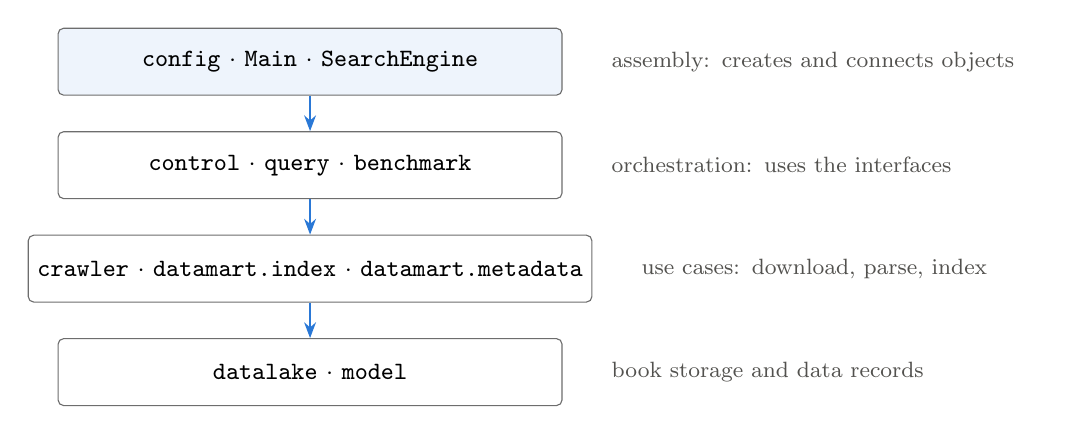
\begin{tikzpicture}[font=\small,
  layer/.style={draw=ink!60,rounded corners=2pt,minimum width=6.4cm,minimum height=0.85cm,fill=white},
  arr/.style={-{Stealth[length=2mm]},thick,draw=accent}]
  \node[layer,fill=notebg] (a) {\code{config} $\cdot$ \code{Main} $\cdot$ \code{SearchEngine}};
  \node[layer,below=0.45cm of a] (b) {\code{control} $\cdot$ \code{query} $\cdot$ \code{benchmark}};
  \node[layer,below=0.45cm of b] (c) {\code{crawler} $\cdot$ \code{datamart.index} $\cdot$ \code{datamart.metadata}};
  \node[layer,below=0.45cm of c] (d) {\code{datalake} $\cdot$ \code{model}};
  \foreach \x/\y in {a/b,b/c,c/d} \draw[arr] (\x) -- (\y);
  \node[right=0.5cm of a,text width=5.2cm,color=muted,font=\footnotesize] {assembly: creates and connects objects};
  \node[right=0.5cm of b,text width=5.2cm,color=muted,font=\footnotesize] {orchestration: uses the interfaces};
  \node[right=0.5cm of c,text width=5.2cm,color=muted,font=\footnotesize] {use cases: download, parse, index};
  \node[right=0.5cm of d,text width=5.2cm,color=muted,font=\footnotesize] {book storage and data records};
\end{tikzpicture}
\caption{Layers. Each one only uses the layers below it.}
\end{figure}

\subsection{Design principles applied throughout}
\begin{table}[H]
\centering\small
\begin{tabularx}{\linewidth}{@{}p{3.1cm} Y Y@{}}
\toprule
Principle & Where & Why \\
\midrule
Programming to interfaces & \code{Datalake}, \code{InvertedIndex}, \code{MetadataRepository}, \code{BookSource} & Changing a structure does not touch its users; tests use doubles (lambdas, in-memory index). \\
Constructor injection & Every class receives its collaborators in the constructor. & Nothing is created behind the scenes; any piece can be replaced in tests. \\
Factory & \code{DatalakeFactory}, \code{InvertedIndexFactory} & One configuration name $\rightarrow$ one implementation, in a single place. \\
Template method & \code{AbstractFileDatalake}: subclasses decide \emph{where}; the base decides \emph{how} a book is written and what counts as saved. & The delicate logic (atomicity) exists only once. \\
Atomic writes & Datalake, JSON index, term files, CSV results: write \code{.tmp}, then rename. & A crash never leaves a half-written file under its final name. \\
Idempotence & \code{save} (upsert), \code{addDocument} (sets), \code{mark*} & Repeating an operation after a failure is safe: nothing is duplicated. \\
Mark after doing & \code{PipelineController}: \code{mark*} only after success. & The control layer never claims something that did not happen; at worst work is repeated. \\
Immutable records & \code{RawBook}, \code{BookLocation}, \code{BookMetadata}, \code{StepResult}, \code{AppConfig} & Data without behaviour, automatic \code{equals}, impossible to modify by accident. \\
\bottomrule
\end{tabularx}
\caption{Design principles and where they appear in the code.}
\end{table}

\subsection{Project organisation}

\subsubsection{Folder tree}
\begin{lstlisting}[style=shell]
Stage_1/
|-- README.md                  overview of the group project
|-- docker-compose.yml         MongoDB 8.2 server shared by the three implementations
|-- shared/                    COMMON CONTRACT (Java, Python and C++)
|   |-- SPEC.md                rules that must not differ between languages
|   |-- book_ids.txt           the 200 books of the dataset, in order
|   |-- queries.txt            AND queries of the index_query benchmark
|   `-- stopwords.txt          English stopwords
|-- sample_dataset/            first 15 books, raw (input) and split (expected output)
`-- java/stage1/               <- the Java implementation (run everything from here)
    |-- pom.xml                Maven: Java 17, JUnit 5, sqlite-jdbc, Jackson, Mongo driver
    |-- config.properties      default configuration (read by AppConfig)
    |-- README.md              user guide of the module
    |-- docs/                  this report; report/ holds its LaTeX source and charts
    |-- src/main/java/es/ulpgc/bigdata/
    |   |-- Main.java          command line: pipeline | search | status | config
    |   |-- SearchEngine.java  assembles the whole system from an AppConfig
    |   |-- model/             RawBook, BookLocation, BookMetadata (records)
    |   |-- crawler/           BookSource, GutenbergClient, LocalFileSource,
    |   |                      BookSplitter, BookDownloader
    |   |-- datalake/          Datalake, AbstractFileDatalake, Book/Range/TimeBasedDatalake
    |   |-- datamart/metadata/ MetadataParser, MetadataRepository, SQLite
    |   |-- datamart/index/    Tokenizer, InvertedIndex + 4 implementations, Indexer
    |   |-- query/             SearchService (AND)
    |   |-- control/           ControlFiles, PipelineController, StepResult, BookIdList
    |   |-- config/            AppConfig, DatalakeFactory, InvertedIndexFactory
    |   `-- benchmark/         BenchmarkRunner, CSV output and the three benchmarks
    |-- src/test/java/...      357 tests (JUnit 5), same package structure
    |-- data/                  (generated, ignored by git) datalake, datamarts, control
    `-- benchmarks/            results/{real,synthetic}/*.csv (committed), work/ (ignored)
\end{lstlisting}

\subsubsection{Size of the code}
\begin{table}[H]
\centering\small
\begin{tabularx}{\linewidth}{@{}l Y@{}}
\toprule
Item & Amount \\
\midrule
Production classes and interfaces & 44 (about 4,800 lines with comments) \\
Test classes & 35 (about 5,200 lines), 357 tests \\
External dependencies & sqlite-jdbc 3.53, jackson-databind 2.22, mongodb-driver-sync 5.13, JUnit 5 \\
\bottomrule
\end{tabularx}
\end{table}

\subsubsection{Where each part of the state lives}
All paths are built by \code{AppConfig} from \code{data.dir} (\code{data/} by default, relative to
\code{java/stage1}). No other class writes a data path; a test fails if one does.

\begin{table}[H]
\centering\small
\begin{tabularx}{\linewidth}{@{}p{2.3cm} Y p{5.4cm}@{}}
\toprule
State & File or database & Written by \\
\midrule
Book text & \code{data/datalake/<structure>/\ldots} & \code{Datalake.save} \\
Metadata & \code{data/datamarts/metadata.db} (table \code{books}) & \code{SqliteMetadataRepository} \\
Monolithic index & \code{data/datamarts/} \code{inverted\_index.json} & \code{MonolithicJsonIndex.flush} \\
Hierarchical index & \code{data/datamarts/inverted\_index/} \code{<L>/<term>.txt} & \code{HierarchicalFolderIndex.flush} \\
Mongo index & database \code{search\_engine}, collection \code{inverted\_index} & \code{MongoInvertedIndex.flush} \\
Progress & \code{data/control/downloaded\_books.txt}, \code{indexed\_books.txt} & \code{ControlFiles.mark*} \\
Benchmark results & \code{benchmarks/results/} \code{java\_<experiment>.csv} & \code{CsvResults.write} \\
\bottomrule
\end{tabularx}
\end{table}

% ================================================================ 3
\section{Design decisions}\label{sec:decisions}

\subsection{Structures selected for the final implementation}
Every structure required by the assignment is implemented and can be selected in
\code{config.properties} without changing code, so the benchmarks compare them on equal terms. The
structures selected in \code{config.properties}, the most efficient ones according to the results of
Section~\ref{sec:bench}, are justified here.

\textbf{Datalake: \code{book} (selected in \code{config.properties}).} It is the most efficient
layout in the experiments that the pipeline actually performs:
\begin{itemize}
  \item \emph{Fastest write:} 1,031 books/s, against 1,006 for \code{range} and 948 for \code{time}.
  \item \emph{Fastest lookup:} the path is computed from the id, 3.3\us{} per book against 8.3\us{}
        for \code{range} and 94.5\us{} for \code{time}, which has to walk its hour folders and gets
        slower as the ingestion runs for more hours.
  \item \emph{Fastest detection of new books:} 1.24~ms, against 2.58 and 2.08~ms.
  \item \emph{Same reliability:} it recovers the 20 interrupted books with no losses or duplicates,
        like the other two. Its recovery time (23.8~ms) is 4~ms slower than \code{time}'s, which is
        negligible.
  \item \emph{One datalake for everything:} the benchmarks read a \code{book} datalake (SPEC 10.1),
        so a single \code{pipeline} run serves both to search and to benchmark.
\end{itemize}
Its drawback is the number of entries in its root folder, one per book (200 here). That is harmless
at this scale, but with tens of thousands of books \code{range} would be the alternative: also a
direct lookup, with at most 2,000 files per folder. \code{time}, the layout suggested by the
assignment, offers traceability and folders bounded by the ingestion rate (20 entries), which would
pay off if a later stage processed only the most recent folders; in Stage~1 nothing does, so its
slower lookup brings no benefit.

\textbf{Inverted index: \code{monolithic} (selected), with \code{mongo} as the scalable option.} At
the scale of this stage (200 books) \code{monolithic} wins every time-based experiment: building
(1.7~s against 11.3 and 14.3~s), querying (4.5\us{} against 48 and 345\us) and adding a book (85~ms
against about 1~s), and it takes the least disk. Its weaknesses are structural: each update
rewrites the whole JSON and the whole index lives on the heap (100~MB for 200 books), both growing
linearly. Beyond roughly 2,000--2,500 real books, or as soon as several processes need the index
(Stage~2), \code{mongo} is the better choice; it is preferred to \code{hierarchical}, which has the
same update cost but wastes 73 times its data size in file-system blocks. Switching is one line of
configuration.

\textbf{Metadata: SQLite with indexes on \code{author} and \code{title}.} The indexes make queries by
author or title about 160 times faster with 100,000 rows, for inserts about 14\% slower. SQLite needs
no server and is more than enough for metadata at this scale.

\subsection{Implementation decisions}
\begin{description}[style=nextline,leftmargin=0pt,itemsep=6pt]
  \item[Interfaces for every storage component.] Callers do not depend on how something is
        implemented: the \code{Indexer} receives an \code{InvertedIndex} and works the same with a
        JSON file, folders or MongoDB. It also enables test doubles and contract tests run against
        every implementation.
  \item[Factories and a single assembly point.] Only the factories know that ``hierarchical'' means a
        \code{HierarchicalFolderIndex} in the \code{inverted\_index} folder, and only
        \code{SearchEngine} connects the pieces. Without them, that mapping would be copied into
        \code{Main} and every benchmark. \code{Main} only parses arguments, connects and prints.
  \item[Write to \code{.tmp}, then rename.] A rename within one file system is atomic: the file under
        its final name is either complete or absent. A crash during a write leaves only a
        \code{.tmp}, which never counts as valid data.
  \item[Header before body.] A book exists only when both files are there. A crash between the two
        leaves the body missing, so the book does not count as stored and is downloaded again.
  \item[Mark the control layer after the operation, never before.] Marking first and then crashing
        would make the control layer claim a book that does not exist, and that book would be lost
        for good. Marking afterwards means the worst case is repeating an operation, which is safe
        because every operation is idempotent (metadata upsert, set-based \code{addDocument},
        \code{\$addToSet} in MongoDB, marks without duplicates, overwriting saves).
  \item[Compute before writing when indexing.] The \code{Indexer} parses and tokenizes everything
        first, so a failure never leaves metadata and index half updated. If power is lost half-way,
        the book is not marked as indexed and is simply indexed again on restart.
  \item[An ASCII-only tokenizer.] Unicode-aware methods such as \code{toLowerCase()} behave
        differently across languages. Treating only A--Z, a--z and 0--9 makes the Java, Python and
        C++ indexes identical, which the reference term counts verify.
  \item[An offline book source.] The sample dataset is served through the same \code{BookSource}
        interface as Gutenberg, so the offline mode exercises exactly the production code path.
\end{description}

% ================================================================ 4
\section{Implementation: packages and classes}
For each class: what it is, its single responsibility, its important methods, and the reason for
its design. The order follows the path of the data.

% ---------------------------------------------------------------- model
\subsection{Package \code{model}: the data that travels}

\cls{RawBook}{record}
A freshly downloaded and split book, before it is stored: \code{id}, \code{header}, \code{body}.
\code{BookSplitter} produces it and \code{Datalake.save} consumes it.
\why{A record is immutable and has \code{equals}, \code{hashCode} and \code{toString} for free:
ideal for data that is only handed from one piece to the next.}

\cls{BookLocation}{record}
Where a book was stored: \code{id}, \code{headerPath}, \code{bodyPath}. It holds paths, not text.
\code{save} and \code{locate} return it.
\why{It separates \emph{where} a book is from \emph{what} it contains: the \code{Indexer} reads the
text only when it needs it.}

\cls{BookMetadata}{record}
A book's metadata: \code{id}, \code{title}, \code{author}, \code{language}, \code{releaseDate} and
the two datalake paths. A field missing from the header is \code{null} (the SPEC says NULL).
\why{Storing the paths in SQLite links the metadata datamart to the datalake: from a search result
one can reach the text.}

% ---------------------------------------------------------------- crawler
\subsection{Package \code{crawler}: fetching and splitting}

\cls{BookSource}{functional interface}
``Where the text of a book comes from'': \code{Optional<String> fetch(int id)}. Empty if the book is
not available (HTTP 404, missing file); an I/O failure is an exception.
\why{It makes the whole system testable without network. In unit tests it is a lambda with
invented books; the end-to-end test uses one that counts its calls; the offline mode uses
\code{LocalFileSource}.}

\cls{GutenbergClient}{class, implements \code{BookSource}}
Downloads \code{https://www.gutenberg.org/cache/epub/<id>/pg<id>.txt} with Java's
\code{HttpClient}. It only downloads: it neither splits nor stores.
\begin{itemize}
  \item Constructor \code{(connectTimeout, requestTimeout)}: the timeouts come from \code{AppConfig}.
  \item \code{fetch}: HTTP 2xx $\rightarrow$ the text; any other status or a network error $\rightarrow$ empty.
\end{itemize}
\why{Single responsibility: if Gutenberg changes its URL, only this class changes.}

\cls{LocalFileSource}{class, implements \code{BookSource}}
The offline counterpart of \code{GutenbergClient}: reads \code{<dir>/pg<id>.txt}, named like the
last part of the download URL (\code{sample\_dataset/raw/}). It returns the bytes decoded as UTF-8
and untouched, \code{\textbackslash r\textbackslash n} included, so everything downstream runs
exactly as online. A missing file is an unavailable book (empty, like a 404); any other read error
is an exception.
\why{Adding the offline mode needed no change in any other class: it is one more
\code{BookSource}, chosen by \code{SearchEngine.openOffline}. The same design exists in the C++
implementation, so both are tested the same way.}

\cls{BookSplitter}{class}
Splits the raw text into header and body as the SPEC defines, and drops the footer. Normalises
\code{\textbackslash r\textbackslash n} to \code{\textbackslash n}. If a marker is missing it
returns empty and the book is discarded.
\begin{itemize}
  \item The body starts at the \emph{end of the line} holding the START marker, not right after
        the pattern, so the title written on that line is not carried into the body.
  \item The END marker is searched for only after the START marker.
\end{itemize}
\why{It is a pure function (no I/O): it is tested with strings, and its output is checked byte by
byte against \code{sample\_dataset/book/}.}

\cls{BookDownloader}{class}
Composite component: \code{fetch} $\rightarrow$ \code{split} $\rightarrow$ \code{save}. Returns the
\code{BookLocation}, or empty if the book is unavailable or has no markers, in which case nothing is
written.
\begin{lstlisting}
return source.fetch(bookId)                            // Optional<String>
        .flatMap(text -> splitter.split(bookId, text))  // Optional<RawBook>
        .map(datalake::save);                           // Optional<BookLocation>
\end{lstlisting}
\why{It does not touch the control files: the caller (\code{PipelineController}) decides. So it can
be reused and tested in isolation.}

% ---------------------------------------------------------------- datalake
\subsection{Package \code{datalake}: storing the books}

\cls{Datalake}{interface}
The contract of any physical layout: \code{name()}, \code{save(RawBook)}, \code{locate(id)},
\code{listBookIds()}. The rest of the system only knows this interface.
\begin{itemize}
  \item \code{locate} only returns complete books (header and body under their final names).
  \item \code{listBookIds} returns sorted ids without repetitions, ignoring \code{.tmp} files and
        any other stray file.
\end{itemize}
\why{A contract test (\code{DatalakeContractTest}, 36 cases) runs against the three
implementations and guarantees that they behave the same.}

\cls{AbstractFileDatalake}{abstract class}
What the three file-based datalakes share. Subclasses only decide \emph{where} each book goes; this
class defines \emph{how} it is written and what counts as a stored book.
\begin{itemize}
  \item \code{writeBook}: header first, then body; a book exists only when both are there.
  \item \code{isCompleteBook}, \code{parseCanonicalId} (rejects \code{0084}, \code{-5} and ids of more
        than 9 digits).
  \item \code{writeAtomically}: create the folder, write \code{x.tmp}, move it to \code{x}:
\end{itemize}
\begin{lstlisting}
static void writeAtomically(Path target, String content) throws IOException {
    Files.createDirectories(target.getParent());
    Path tmp = target.resolveSibling(target.getFileName() + TMP_SUFFIX);
    try {
        Files.writeString(tmp, content, StandardCharsets.UTF_8);
        try {
            Files.move(tmp, target, ATOMIC_MOVE, REPLACE_EXISTING);
        } catch (AtomicMoveNotSupportedException e) {
            Files.move(tmp, target, REPLACE_EXISTING);   // no atomic move on this file system
        }
    } catch (IOException e) {
        Files.deleteIfExists(tmp);                       // do not leave garbage if something fails
        throw e;
    }
}
\end{lstlisting}
\why{Template method pattern. The delicate part (atomicity, the definition of a complete book) is
written once and cannot diverge between layouts.}

\cls{BookBasedDatalake}{class, layout \code{book}}
One folder per book: \code{<root>/<id>/header.txt} and \code{body.txt}.
\why{The simplest layout: \code{locate} computes the path directly. Drawback: the root holds as
many entries as there are books (200 in the benchmark; a problem with millions).}

\cls{RangeBasedDatalake}{class, layout \code{range}}
Folders by ranges of 1000 ids: \code{01000-01999/1342.body.txt}.
\why{The path is also computed from the id (direct lookup), and no folder can exceed 2,000 files.
\code{listBookIds} also checks that each file is in its correct range.}

\cls{TimeBasedDatalake}{class, layout \code{time}}
Folders by date and hour of download: \code{20260930/19/84.body.txt}. It receives a \code{Clock}
so tests and benchmarks can simulate time.
\begin{itemize}
  \item \code{save} reads the clock once, so header and body land in the same folder even if the
        hour changes in between.
  \item \code{locate} cannot compute the path: it walks the folders from newest to oldest. If an id
        appears twice, the newest copy wins.
  \item Patterns \code{yyyyMMdd} and \code{HH} (not \code{YYYY}, the ISO week year, nor \code{hh},
        the 12-hour clock).
\end{itemize}
\why{It records when each book arrived, which suits incremental ingestion, at the cost of a slow
lookup that the benchmark makes visible.}

\cls{DatalakeStats}{record}
A snapshot of a folder: directories, files, bytes, and the largest number of entries in one
directory. Used by the benchmarks.

% ---------------------------------------------------------------- metadata
\subsection{Package \code{datamart.metadata}: metadata in SQLite}

\cls{MetadataParser}{class}
Extracts \code{title}, \code{author}, \code{release\_date} and \code{language} from the header with
the SPEC's regular expressions. It reads no files: it receives the text and the
\code{BookLocation} (for the id and paths).
\begin{itemize}
  \item \code{MULTILINE} regexes: \code{\^{}} and \code{\$} match the start and end of each line.
  \item \code{release\_date} drops what is inside brackets: ``March 3, 2001 [eBook \#10]''
        $\rightarrow$ ``March 3, 2001''.
  \item A value that is empty after trimming is treated as missing (\code{null}).
\end{itemize}

\cls{MetadataRepository}{interface}
Metadata store: \code{save}, \code{saveAll}, \code{findById}, \code{findByAuthor},
\code{findByTitle}, \code{count}, \code{clear}, \code{close}.
\begin{itemize}
  \item \code{save} and \code{saveAll} are idempotent (saving an id again updates it); \code{saveAll}
        is all-or-nothing.
  \item Searches use exact equality and return results sorted by id.
\end{itemize}
\why{\code{close()} is redeclared without \code{throws Exception}, so the repository can be used in
try-with-resources without catching anything.}

\cls{SqliteMetadataRepository}{class}
JDBC implementation over one SQLite file. It keeps one connection open until \code{close()} and
creates the folder and the schema when opened.
\begin{itemize}
  \item Upsert: \code{INSERT \ldots{} ON CONFLICT(book\_id) DO UPDATE}, so re-indexing a book neither
        fails nor duplicates it.
  \item \code{saveAll}: one transaction with \code{addBatch}/\code{executeBatch} and a single commit;
        rollback if anything fails.
  \item Always \code{PreparedStatement}, never concatenated SQL (no injection, no quoting bugs).
\end{itemize}
\why{\code{SQLException} is wrapped in \code{MetadataRepositoryException}, so callers do not depend
on JDBC.}

\cls{SqliteSchema}{utility class}
The \code{CREATE TABLE books} and the indexes \code{idx\_books\_author} and \code{idx\_books\_title},
all with \code{IF NOT EXISTS} so they run on every open. It also builds the JDBC URL.

\cls{MetadataRepositoryException}{unchecked exception}
An error of the metadata store; wraps the original \code{SQLException}.

% ---------------------------------------------------------------- index
\subsection{Package \code{datamart.index}: the inverted index}
An inverted index stores, for each term, the list of books that contain it (its \emph{posting
list}). It is ``inverted'' because a book contains terms, and the index turns that around: from the
term to the books. Example: \code{whale} $\rightarrow$ [84, 2701], \code{island} $\rightarrow$
[76, 84, 2701, \ldots].

\cls{Tokenizer}{class}
Turns text into terms following the SPEC. \code{tokenize} returns every token with repetitions;
\code{uniqueTerms} returns each term once, in order of first appearance (what a book contributes);
\code{fromStopwordsFile} loads \code{shared/stopwords.txt}. Both share one loop:
\begin{lstlisting}
for (int i = 0; i < text.length(); i++) {
    char c = text.charAt(i);
    if (c >= 'A' && c <= 'Z') {
        current.append((char) (c + ('a' - 'A')));     // ASCII uppercase -> lowercase
    } else if ((c >= 'a' && c <= 'z') || (c >= '0' && c <= '9')) {
        current.append(c);
    } else {
        emit(current, sink);                          // separator: closes the token
    }
}
emit(current, sink);                                  // the text may end in the middle of a token
\end{lstlisting}
\code{emit} drops tokens shorter than 2 characters and stopwords.
\why{It uses neither \code{toLowerCase()} nor \code{Character.isLetter()}: they follow Unicode
rules that the C++ implementation cannot reproduce byte for byte. That is why ``café'' gives
``caf'' in every language, and why the term counts match exactly across implementations.}

\cls{InvertedIndex}{interface}
Contract: \code{name}, \code{addDocument(id, terms)}, \code{postings(term)}, \code{flush},
\code{clear}, \code{diskUsageBytes}, \code{close}.
\begin{itemize}
  \item \code{postings} is sorted, without repetitions and unmodifiable; empty if the term does not
        exist. It sees what was added even before \code{flush}.
  \item \code{addDocument} is idempotent; \code{clear} also empties the disk.
  \item After \code{flush}, closing and reopening keeps everything.
\end{itemize}
\why{\code{InvertedIndexContractTest} (33 cases) checks these rules on every implementation.}

\begin{table}[H]
\centering\small
\begin{tabularx}{\linewidth}{@{}l Y Y@{}}
\toprule
Implementation & What \code{flush} does & Where the index lives \\
\midrule
\code{InMemoryInvertedIndex} & Nothing (not persistent). & \code{HashMap<String, TreeSet<Integer>>} in memory. \\
\code{MonolithicJsonIndex} & Rewrites the whole JSON (temp file + move). & All in memory (\code{TreeMap}); fully loaded when opened. \\
\code{HierarchicalFolderIndex} & Rewrites only the files of the terms that changed. & One file per term; only pending changes in memory. \\
\code{MongoInvertedIndex} & One \code{bulkWrite} with an upsert + \code{\$addToSet} per term. & In the MongoDB server; only pending changes in memory. \\
\bottomrule
\end{tabularx}
\caption{The four index implementations.}
\end{table}

\cls{InMemoryInvertedIndex}{class, structure \code{memory}}
A map term $\rightarrow$ \code{TreeSet} of ids: \code{computeIfAbsent(term).add(id)}, and the
\code{TreeSet} keeps ids sorted and unique. It is the ``perfect'' reference in tests and benchmarks,
and exposes \code{terms()} and \code{termCount()} to check the reference values.

\cls{MonolithicJsonIndex}{class, structure \code{monolithic}}
The whole index in a \code{TreeMap<String, TreeSet<Integer>>}, and on disk one JSON file written
with Jackson. Opening loads the whole file; \code{flush} rewrites it entirely if anything changed
(\emph{dirty} flag).
\begin{itemize}
  \item A corrupt JSON throws an exception instead of starting empty: otherwise the next
        \code{flush} would overwrite the good index with an empty one.
\end{itemize}
\why{Very fast queries (everything in memory) and one simple file; but each update costs as much as
writing the whole index, and the whole index must fit in RAM.}

\cls{HierarchicalFolderIndex}{class, structure \code{hierarchical}}
One file per term, one id per line: \code{B/boat.txt}. The folder is the term's first letter in
uppercase; terms starting with a digit go to that digit's folder.
\begin{itemize}
  \item \code{addDocument} accumulates in \code{pending}; \code{flush} reads, merges and atomically
        rewrites only the files of the terms touched.
  \item \code{postings} reads only the requested term's file and adds what is pending.
  \item Validates that the term matches \code{[a-z0-9]+} (no odd paths, no problems on
        case-insensitive file systems).
\end{itemize}
\why{Adding a book only touches its own terms, and memory use is minimal; in exchange there are
many thousands of small files (much space wasted in 4~KB blocks) and every query is a disk read.}

\cls{MongoInvertedIndex}{class, structure \code{mongo}}
Documents \code{\{"term": "boat", "postings": [10, 20]\}} with a unique index on \code{term}. It
accumulates in memory and \code{flush} sends everything in one unordered \code{bulkWrite}.
\begin{itemize}
  \item \code{\$addToSet} with \code{\$each}: adds only ids not already present (idempotent).
  \item MongoDB does not guarantee array order: \code{postings} sorts when reading.
  \item \code{diskUsageBytes} = \code{storageSize} + \code{totalIndexSize}, after an \code{fsync}
        (without it, WiredTiger may not have written the data yet).
  \item 3-second server selection timeout if MongoDB does not answer.
\end{itemize}
\why{Cheap updates and a server that handles caching, compression and concurrency; the cost is a
network round trip for every query term.}

\cls{Indexer}{class}
The bridge from the datalake to the datamarts for one book: \code{index(id)}.
\begin{enumerate}
  \item Read and compute everything without writing anything (header, body, metadata, terms).
  \item Save the metadata.
  \item \code{addDocument} and \code{flush}.
\end{enumerate}
It returns empty, and touches nothing, if the book is not in the datalake.
\why{Computing before writing avoids half-done states. Metadata goes before the index: a book with
metadata but no index entry is invisible, while the opposite would return results without a
title.}

% ---------------------------------------------------------------- query
\subsection{Package \code{query}: the search}

\cls{SearchService}{class}
AND search: query $\rightarrow$ terms (same tokenizer) $\rightarrow$ posting lists $\rightarrow$
intersection. It never reads books.
\begin{itemize}
  \item If one term has no postings it returns \code{[]} without asking for the rest (each request
        costs a disk read or a round trip in \code{hierarchical} and \code{mongo}).
  \item It sorts the lists from shortest to longest: the result can never be longer than the
        shortest list.
\end{itemize}
\begin{lstlisting}
static List<Integer> intersect(List<Integer> a, List<Integer> b) {
    List<Integer> result = new ArrayList<>(Math.min(a.size(), b.size()));
    int i = 0, j = 0;
    while (i < a.size() && j < b.size()) {
        int x = a.get(i), y = b.get(j);
        if (x == y) { result.add(x); i++; j++; }   // in both: keep it, advance both
        else if (x < y) i++;                       // x cannot be in b
        else j++;                                  // y cannot be in a
    }
    return result;
}
\end{lstlisting}
\why{Two pointers over sorted lists take at most $n+m$ steps, $O(n+m)$. The service works the same
with any \code{InvertedIndex}.}

% ---------------------------------------------------------------- control
\subsection{Package \code{control}: progress and recovery}

\cls{BookIdList}{utility class}
Reads a list of book ids (\code{shared/book\_ids.txt}, or \code{sample\_dataset/book\_ids.txt}
offline): ids in order, without repetitions; empty lines and \code{\#} lines ignored. A line that is
not an id is an error, because the file is written by hand and a typo must not go unnoticed.

\cls{ControlFiles}{class}
The two control files as sets: \code{readyToIndex} = downloaded $-$ indexed.
\begin{itemize}
  \item Loaded once; each mark is appended to the end of the file, first on disk and then in memory.
  \item When loading, only complete lines (ending in \code{\textbackslash n}) count; a half-written
        tail is trimmed so the next append cannot form a false id (``13'' + ``84\textbackslash n''
        = ``1384'').
\end{itemize}

\cls{PipelineController}{class}
Decides what to do next and asks whoever knows how to do it: it does not download, parse or index.
\begin{itemize}
  \item \code{step()}: at most one operation. Priority: index what is downloaded; otherwise download
        the next book of the dataset; otherwise \code{IDLE}.
  \item Marks the control layer only after the operation has succeeded.
  \item Books that fail are skipped for the rest of the run (\code{skippedThisRun}, in memory only)
        and retried after a restart.
  \item \code{runUntilIdle(max)}: repeats steps until \code{IDLE} or the limit.
\end{itemize}
\why{Everything needed to continue is in the control files; the process may die at any moment
without losing or duplicating anything.}

\cls{StepResult}{record}
What one step did: \code{action} (\code{INDEXED}, \code{DOWNLOADED}, \code{NOT\_AVAILABLE},
\code{MISSING\_FROM\_DATALAKE}, \code{DOWNLOAD\_FAILED}, \code{INDEX\_FAILED}, \code{IDLE}),
\code{bookId}, and \code{detail} (the error message).

% ---------------------------------------------------------------- config
\subsection{Package \code{config} and assembly}

\cls{AppConfig}{record}
All the configuration, and the only place that builds paths (\code{datalakeDir()},
\code{metadataDb()}, \code{monolithicIndexFile()}, \code{controlDir()}, \code{sampleRawDir()},
\code{sampleBookIdsFile()}\ldots).
\begin{itemize}
  \item \code{load()}: defaults $<$ file $<$ \code{MONGO\_URI} $<$ \code{-D}.
  \item Validates in the constructor: an unknown structure, an unknown key or a timeout $\le 0$
        fails at start-up, not half-way through a run.
  \item \code{withDataDir}: the same configuration with another data folder (benchmarks work apart).
\end{itemize}
\why{A test walks \code{src/main/java} and fails if a data path appears outside \code{AppConfig}.}

\cls{DatalakeFactory}{utility class}
Maps \code{"book"} | \code{"range"} | \code{"time"} to the matching class: the only
\code{new XxxDatalake} of the application. An unknown name throws an exception that lists the valid
options.

\cls{InvertedIndexFactory}{utility class}
Maps \code{"monolithic"} | \code{"hierarchical"} | \code{"mongo"} | \code{"memory"} to an
\code{InvertedIndex}, with the paths and connection data supplied by \code{AppConfig}.

\cls{SearchEngine}{class}
The complete system assembled from an \code{AppConfig}: datalake, metadata, index, control,
pipeline and search. It is the only place where the pieces are connected.
\begin{itemize}
  \item \code{open(config)}: with the real Project Gutenberg (used by \code{Main}).
  \item \code{openOffline(config)}: with \code{LocalFileSource} over \code{sample\_dataset/raw/} and
        the sample's 15 ids (used by \code{Main} with \code{-{}-offline} and by \code{SampleDatasetTest}).
  \item \code{open(config, source)} and \code{open(config, source, bookIdsFile)}: with any
        \code{BookSource} (the end-to-end test, without network).
  \item \code{close()}: closes the index and SQLite (the second even if the first fails).
\end{itemize}
\why{If the tests assembled the pieces themselves, they would test their own assembly and not the
program's. With \code{SearchEngine}, the tests and \code{Main} share exactly the same wiring.}

\cls{Main}{class}
Thin command-line layer: parses \code{[--config file] command [--offline]}, loads \code{AppConfig},
asks \code{SearchEngine} for the system and prints the results. No business logic. Configuration
and argument errors $\rightarrow$ message and exit code 2.

% ---------------------------------------------------------------- benchmark
\subsection{Package \code{benchmark}}

\cls{BenchmarkRunner}{class}
Repeats a task and measures it: for each repetition it runs \code{setup()} (not timed) and then
\code{task()} between two \code{System.nanoTime()} calls. It discards the warm-ups and returns one
row per measured run.
\why{\code{nanoTime} is a monotonic clock meant for intervals; \code{currentTimeMillis} is wall
time and can jump (NTP adjustments).}

\cls{BenchmarkRow}{record}
One row of the common CSV. Validates that text fields contain no commas or quotes (so the CSV needs
no escaping and Python and C++ read it the same way) and formats numbers with a decimal point and at
most 3 decimals.

\cls{CsvResults}{utility class}
Writes \code{benchmarks/results/java\_<experiment>.csv} at once, with temp file + move: if a
benchmark fails, the previous CSV is left untouched.

\cls{BenchmarkBooks}{utility class}
Where benchmark books come from (never the network): an existing datalake (sorted by id, as
SPEC 10.1 requires), \code{synthetic} (16 words, for the datalake), or \code{syntheticZipf} (30,000
words with a Zipf distribution, for the index; query words at ranks 10, 40, 90\ldots{} so they have
different selectivities).

\cls{SimulatedClock}{class}
A clock that advances 6 minutes each time it is read: a reproducible ingestion of 10 books per hour,
so the \code{time} layout spreads books over folders as it would in reality.

\cls{DatalakeBenchmark, MetadataBenchmark, IndexBenchmark}{classes}
The three benchmark programs, one \code{main} each. They are described in Section~\ref{sec:bench}.

% ================================================================ 5
\section{Testing strategy}
357 JUnit~5 tests at four levels. The 12 that need MongoDB are skipped (not failed) when no server
is reachable, and pass with one.

\begin{table}[H]
\centering\small
\begin{tabularx}{\linewidth}{@{}l Y Y@{}}
\toprule
Level & What it checks & Examples (number of tests) \\
\midrule
Unit & One class in isolation, with doubles for its collaborators. & \code{TokenizerTest} (17), \code{MetadataParserTest} (14), \code{BookSplitterTest} (5), \code{ControlFilesTest} (13), \code{SearchServiceTest} (14), \code{LocalFileSourceTest} (3) \\
Contract & The same tests against every implementation of an interface. & \code{DatalakeContractTest} (36), \code{InvertedIndexContractTest} (33) \\
Integration & Several real pieces together, with real disk and databases. & \code{IndexerTest} (9), \code{PipelineControllerTest} (11), \code{SqliteMetadataRepositoryTest} (15), \code{MongoInvertedIndexTest} (10) \\
System & The whole program, assembled as in \code{Main}, without network. & \code{EndToEndTest} (6), \code{SampleDatasetTest} (1) \\
\bottomrule
\end{tabularx}
\caption{Test levels.}
\end{table}

\subsection{The end-to-end test}
\begin{enumerate}
  \item Three invented books in the real Gutenberg format (\code{\textbackslash r\textbackslash n},
        markers, licence footer), ids 10, 1500 and 2003, in three different ranges.
  \item A fake \code{BookSource} that counts its calls: the test does not depend on the Internet.
  \item \code{SearchEngine.open(config, fake)} $\rightarrow$ pipeline until \code{IDLE}: 3 downloads
        + 3 indexings.
  \item Metadata: title, author, language, release date without ``[eBook \#10]'', and the body path
        stored in SQLite is the datalake's.
  \item Ten AND queries with known answers: several terms, uppercase and punctuation, numbers, only
        stopwords, and words that appear only in the title, author or footer (they must not be
        found: only the body is indexed).
  \item Everything is closed, the location of each part of the state on disk is checked, and the
        system is reopened with a source that fails if called. The queries must return identical
        results and nothing is downloaded again.
\end{enumerate}
It is repeated with \code{time}+\code{monolithic}, \code{book}+\code{hierarchical},
\code{range}+\code{monolithic} and \code{book}+\code{mongo}. A second test simulates the process
dying without calling \code{close()}: the state survives, because it is made persistent at each
\code{flush} and each mark, not when closing.

To check that the test is useful, two faults were introduced on purpose in the assembly:
forgetting the stopwords (the query ``the of'' returned [2003]) and storing the control files in a
different folder on each start (``the book 10 was downloaded again after the restart''). The test
caught both.

\subsection{The sample dataset test}
\code{SampleDatasetTest} runs \code{SearchEngine.openOffline} on the real 15 books of
\code{sample\_dataset/} with the \code{book} layout and the in-memory index. It checks the 30 step
results, compares every stored \code{header.txt} and \code{body.txt} byte by byte with
\code{sample\_dataset/book/}, counts exactly 30,396 terms and 89,727 postings, and checks the answer
to ``whale island''. It is the test that ties the Java implementation to the group's shared
reference data.

% ================================================================ 6
\section{Setup and execution}

\subsection{Requirements}
\begin{itemize}
  \item JDK 17 or newer (the \code{pom.xml} compiles for 17; tested with OpenJDK 21) and Maven 3.
  \item MongoDB only for the \code{mongo} index or its benchmark. Without a server, its tests are
        skipped (not failed) and the benchmark leaves it out with a warning. The group's server is
        started from the repository root with \code{docker compose up -d} (MongoDB 8.2 on
        \code{127.0.0.1:27017}).
  \item Network only for the online \code{pipeline} command. Tests, benchmarks and the offline mode
        do not use it.
\end{itemize}

\subsection{Build and test}
All commands are run from \code{java/stage1/}.
\begin{lstlisting}[style=shell]
mvn package          # compiles and runs the 357 tests (12 skipped without MongoDB)
mvn -q dependency:build-classpath -Dmdep.outputFile=target/classpath.txt
CP="target/classes:$(cat target/classpath.txt)"
\end{lstlisting}
The \code{pom.xml} does not build a fat jar, so the program runs from the compiled classes plus the
library classpath saved in \code{\$CP}. \code{mvn exec:java -Dexec.mainClass=es.ulpgc.bigdata.Main
-Dexec.args="\ldots"} also works, without the classpath step.

\subsection{Quick test without network: the sample dataset}\label{sec:quick}
The folder \code{sample\_dataset/} at the repository root holds the first 15 books of the dataset
in two forms: \code{raw/pg<ID>.txt}, the files exactly as Project Gutenberg serves them (the
\emph{input} of the pipeline), and \code{book/<ID>/header.txt} and \code{body.txt}, the same books
already split (the \emph{expected output}). With the \code{-{}-offline} option, the pipeline reads
the raw files instead of downloading them. Everything after fetching a book is the same code as
online.

\begin{lstlisting}[style=shell]
java -cp "$CP" es.ulpgc.bigdata.Main pipeline 30 --offline   # 15 downloads + 15 indexings
java -cp "$CP" es.ulpgc.bigdata.Main search whale island
java -cp "$CP" es.ulpgc.bigdata.Main status --offline
\end{lstlisting}
Expected output (the program's messages are in Spanish):
\begin{lstlisting}[style=shell]
offline: libros leídos de .../Stage_1/sample_dataset/raw
datalake=book  index=monolithic
DOWNLOADED 1342
INDEXED 1342
...
DOWNLOADED 76
INDEXED 76

3 libros para "whale island" (index=monolithic)
  76  Adventures of Huckleberry Finn
  84  Frankenstein; or, the modern prometheus
  2701  Moby Dick; Or, The Whale

dataset:     15 (sample_dataset)
descargados: 15
indexados:   15
pendientes:  []
\end{lstlisting}

Every structure can be tried offline with the usual \code{-D} options (for example
\code{-Dindex.structure=hierarchical}), and \code{-Ddata.dir=/tmp/sample} keeps the run apart from \code{data/}. The raw files are
byte-identical to what Gutenberg serves, so a later online \code{pipeline} finds those 15 books
already done and only downloads the other 185.

\begin{note}
\textbf{Automatic check.} \code{SampleDatasetTest}, run by \code{mvn package}, runs this offline
pipeline and verifies that (1) the split of every raw file is byte-identical to
\code{sample\_dataset/book/<ID>/}, (2) the index has exactly \textbf{30,396 distinct terms and
89,727 postings}, the reference values of the sample, and (3) ``whale island'' returns books 76,
84 and 2701, the same answer as the C++ implementation.
\end{note}

\subsection{Commands}
\begin{lstlisting}[style=shell]
java -cp "$CP" es.ulpgc.bigdata.Main [--config file.properties] <command>
\end{lstlisting}
\begin{table}[H]
\centering\small
\begin{tabularx}{\linewidth}{@{}l Y c@{}}
\toprule
Command & What it does & Network \\
\midrule
\code{pipeline [steps]} & Runs up to \code{steps} steps (default 10). A step is \emph{one} download or \emph{one} indexing, so each book needs two steps: \code{pipeline 400} processes the 200 books. It can be interrupted and relaunched: it resumes where it stopped. & yes \\
\code{pipeline [steps] -{}-offline} & The same pipeline over the 15 books of \code{sample\_dataset/}, read from \code{raw/}. & no \\
\code{search <words\ldots>} & AND search with the active index; prints id and title (from SQLite). & no \\
\code{status [-{}-offline]} & Dataset size, downloaded, indexed and still pending indexing. & no \\
\code{config} & The effective configuration, after applying the file, the environment and \code{-D}. & no \\
\bottomrule
\end{tabularx}
\end{table}

Each line printed by \code{pipeline} is one step result: \code{DOWNLOADED}, \code{INDEXED},
\code{NOT\_AVAILABLE} (no such book, or no START/END markers), \code{DOWNLOAD\_FAILED},
\code{INDEX\_FAILED} or \code{MISSING\_FROM\_DATALAKE}. Only the first two are recorded in the
control layer. A book that fails is skipped for the rest of the run and retried in the next one.
A configuration or argument error stops the program with a clear message and exit code 2.

\subsection{Configuration: changing structures without touching code}
Each value comes from four sources, and later ones win: (1) the defaults in \code{AppConfig},
(2) \code{config.properties} or the file given with \code{-{}-config}, (3) the \code{MONGO\_URI}
environment variable, (4) \code{-Dkey=value} system properties.

\begin{lstlisting}[style=shell]
data.dir = data
shared.dir = ../../shared
sample.dir = ../../sample_dataset           # used by --offline
benchmarks.dir = benchmarks
datalake.structure = book                   # book | range | time
index.structure = monolithic                # monolithic | hierarchical | mongo | memory
mongo.uri = mongodb://localhost:27017
mongo.database = search_engine
mongo.collection = inverted_index
http.connect.timeout.seconds = 10
http.request.timeout.seconds = 15
\end{lstlisting}
\begin{lstlisting}[style=shell]
java -cp "$CP" -Ddatalake.structure=book -Dindex.structure=hierarchical es.ulpgc.bigdata.Main pipeline 400
\end{lstlisting}
A misspelt value (\code{index.structure=hierarchcal}), an unknown key or a timeout of 0 stops the
program at start-up with a message that lists the valid options.

\subsection{Running the benchmarks}
The benchmarks never use the network. The 200 real books are downloaded once by the pipeline into a
\code{book} datalake, and that folder is passed to the datalake and index benchmarks:
\begin{lstlisting}[style=shell]
java -cp "$CP" -Ddatalake.structure=book es.ulpgc.bigdata.Main pipeline 400
java -cp "$CP" es.ulpgc.bigdata.benchmark.DatalakeBenchmark data/datalake/book
java -cp "$CP" es.ulpgc.bigdata.benchmark.IndexBenchmark 50,100,200 data/datalake/book
java -cp "$CP" es.ulpgc.bigdata.benchmark.MetadataBenchmark 1000,10000,100000
\end{lstlisting}
Without the datalake argument, \code{DatalakeBenchmark} and \code{IndexBenchmark} use synthetic
books. \code{sample\_dataset/book} is also a valid datalake argument for a quick run. The
benchmarks should be run with plain \code{java} rather than through Maven, because
\code{index\_memory} measures the heap of the JVM it runs in. Each run overwrites
\code{benchmarks/results/java\_*.csv}; the committed runs are archived in \code{results/real/} and
\code{results/synthetic/}.

% ================================================================ 7
\section{Benchmarks and results}\label{sec:bench}

\subsection{Methodology}
\begin{itemize}
  \item \textbf{Warm-ups and measured runs:} 2 discarded repetitions (they warm up the JIT, disk
        caches and connections) and 5 measured ones. Tables give the \textbf{median} of the 5, which
        resists outliers such as a garbage-collector pause.
  \item \textbf{Setup outside the measurement:} clearing, preparing data and opening connections
        happen in \code{setup()}, which is not timed. A test checks this with a deliberately slow
        setup.
  \item \textbf{Same data for everyone:} each structure receives exactly the same list, in the same
        order.
  \item \textbf{No network:} real books are read from a \code{book} datalake already filled by the
        pipeline; synthetic data is generated with a fixed seed.
  \item \textbf{Growing sizes:} each N is the N books with the lowest ids, so every N is a prefix
        of the next and all languages measure the same books (SPEC 10.1).
  \item \textbf{Verification:} after measuring, the result is checked (books found, rows inserted,
        posting lists equal to an in-memory reference). A benchmark that measures something wrong
        fails instead of writing numbers.
  \item \textbf{Output:} one CSV per experiment in the common SPEC format, comparable with Python
        and C++.
\end{itemize}

All results use the common CSV format of the SPEC, so they can be compared directly with the
Python and C++ implementations of the group; this report discusses the Java results.

\begin{note}
\textbf{Environment.} Linux, 12 threads, 15~GB RAM, NVMe SSD, OpenJDK~21, MongoDB~8.2 in Docker
(local). Absolute values depend on the machine; what matters are the ratios and how they change as
N grows.
\end{note}

\subsection{Data: real and synthetic books}
The main results use the \textbf{real} books: they are what the SPEC requires (the same books in
the three languages) and the only data with a genuine vocabulary. The synthetic results of the first
version are kept as a reference and compared with the real ones in Section~\ref{sec:realsyn}.

\begin{table}[H]
\centering\small
\begin{tabularx}{\linewidth}{@{}l Y Y@{}}
\toprule
Benchmark & Real data (\code{results/real/}) & Synthetic data (\code{results/synthetic/}) \\
\midrule
Datalake & The 200 books of \code{shared/book\_ids.txt}, downloaded from Gutenberg (129.0~MB). & 200 books of 300~KB with 16 distinct words (61.5~MB). \\
Index & Prefixes of 50, 100 and 200 of those books. With 200: 129,356 terms and 1,581,064 postings. & Books of 5,000 words drawn with Zipf from 30,000. With 200: 29,716 terms. \\
Metadata & --- (200 rows are too few to see SQLite scale). & Generated rows (SPEC 10.2): 1,000, 10,000 and 100,000. \\
\bottomrule
\end{tabularx}
\end{table}

The 200 ids are the 15 original books plus the most downloaded English books of Gutenberg and
classic fiction; all of them were checked to download with both markers. Many are classics with low
ids: 110 of the 200 are below 1,000, which shows in the \code{range} layout. The term and posting
counts match the reference values of SPEC 10.1 exactly (58,834 / 78,820 / 129,356 terms for
N = 50 / 100 / 200).

\subsection{Datalake benchmark}
Data: the 200 real books (129.0~MB, the same bytes in the three layouts). The \code{time} layout
uses the \code{SimulatedClock} (10 books per hour).

\begin{table}[H]
\centering\small
\begin{tabularx}{\linewidth}{@{}l Y l@{}}
\toprule
Experiment & What exactly is measured & Metrics \\
\midrule
\code{datalake\_write} & Saving the N books into an empty datalake (setup: delete the folder). & elapsed (ms), throughput (books/s) \\
\code{datalake\_lookup} & \code{locate()} of every id, in a fixed random order (seed 42). & elapsed, per\_lookup (\us) \\
\code{datalake\_incremental} & With 90\% known and 10\% new: \code{listBookIds()} minus the known ones. & elapsed, detected \\
\code{datalake\_recovery} & 1 in 10 books has its body left as \code{.tmp} (simulated crash); detecting the missing ones and saving them again. & elapsed, recovered, lost, duplicates \\
\code{datalake\_storage} & After saving everything: files, folders, max entries per folder, bytes and allocated bytes. & files, directories, \ldots \\
\bottomrule
\end{tabularx}
\end{table}

\begin{figure}[H]
\centering
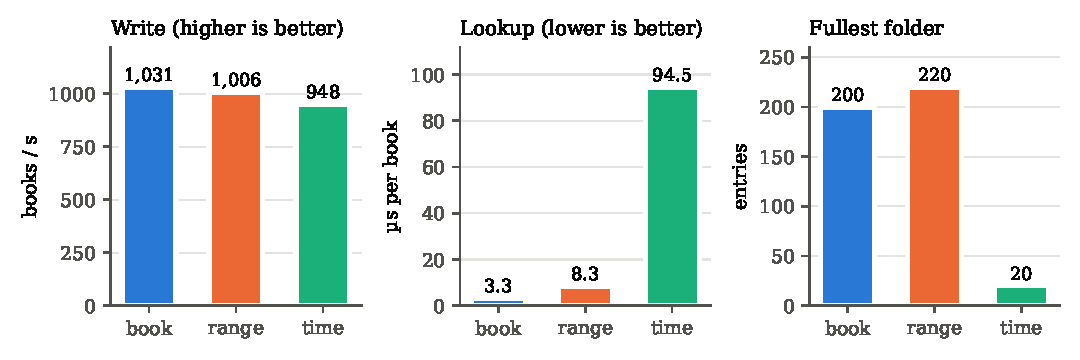
\includegraphics[width=\linewidth]{figures/datalake.pdf}
\caption{Datalake with the 200 real books (median of 5 runs).}
\end{figure}

\begin{table}[H]
\centering\small
\begin{tabular}{@{}lrrr@{}}
\toprule
Metric & \code{book} & \code{range} & \code{time} \\
\midrule
Total write (ms) & 194.0 & 198.8 & 210.9 \\
Write (books/s) & 1,031 & 1,006 & 948 \\
Lookup per book (\us) & 3.3 & 8.3 & 94.5 \\
Detect new books (ms) & 1.24 & 2.58 & 2.08 \\
Recovery (ms) & 23.8 & 25.2 & 19.8 \\
Books recovered / lost / duplicated & 20 / 0 / 0 & 20 / 0 / 0 & 20 / 0 / 0 \\
Folders & 200 & 47 & 21 \\
Max entries in one folder & 200 & 220 & 20 \\
Data / allocated (MB) & 129.0 / 130.9 & 129.0 / 130.3 & 129.0 / 130.2 \\
\bottomrule
\end{tabular}
\end{table}

\textbf{Discussion.}
\begin{itemize}
  \item \textbf{Lookup:} \code{book} (3.3\us) and \code{range} (8.3\us) compute the path from the id:
        one file check. \code{time} (94.5\us, about 29 times \code{book}) cannot compute it and walks
        the hour folders from newest to oldest; its cost grows with the number of ingestion hours.
  \item \textbf{Write:} the three take almost the same time, within 9\% (194--211~ms, about 1,000
        books/s): writing 129~MB and the atomic renames dominate, not the folder layout. With
        synthetic data the order between them was different (\code{time} was fastest), a sign that
        these differences are noise.
  \item \textbf{Incremental and recovery:} all three detect exactly the 20 new books (10\%) and
        recover the 20 damaged ones without losses or duplicates, thanks to the single definition of
        a ``complete book'' (a \code{.tmp} never counts).
  \item \textbf{Storage:} the bytes are identical, but 110 of the 200 ids are between 0 and 999, so
        \code{range} puts 110 books (220 files) into \code{00000-00999}: its fullest folder holds
        more entries than the root of \code{book}. \code{range} guarantees at most 2,000 files per
        folder but does not spread well when ids are concentrated. \code{time} limits each folder to
        what arrives in one hour (20 files), whatever the ids.
  \item \textbf{Conclusion:} \code{book} or \code{range} when books are looked up by id (the normal
        case when indexing and showing results); \code{time} when processing in arrival order
        matters.
\end{itemize}

\subsection{Metadata benchmark}
Data: synthetic rows as SPEC 10.2 defines them: book $i$ has author ``Author $\lfloor i/10\rfloor$''
and title ``Title $\lfloor i/2\rfloor$''. Each author always has 10 books and each title 2,
whatever N is: as N grows, only the table grows, not the size of each answer. Header parsing is not
timed. Two variants are compared: \code{sqlite} (with the SPEC's indexes on \code{author} and
\code{title}) and \code{sqlite\_no\_index} (without them; \code{book\_id} is still the PRIMARY KEY).

This is the only benchmark that stays synthetic, on purpose: it reads ready-made rows, not books, so
the real text has no influence, and the difference between an index and a full scan only appears
with thousands of rows, not 200.

\begin{table}[H]
\centering\small
\begin{tabularx}{\linewidth}{@{}l Y l@{}}
\toprule
Experiment & What is measured & Metrics \\
\midrule
\code{metadata\_insert} & \code{saveAll} into an empty database, in batches of 1,000 (one transaction each). & elapsed (ms), throughput (rows/s) \\
\code{metadata\_query} & 1,000 queries of each kind, with existing values (fixed seed); each kind measured separately. & \code{find\_by\_*} (ms) and \code{*\_avg} (\us) \\
\bottomrule
\end{tabularx}
\end{table}

\begin{figure}[H]
\centering
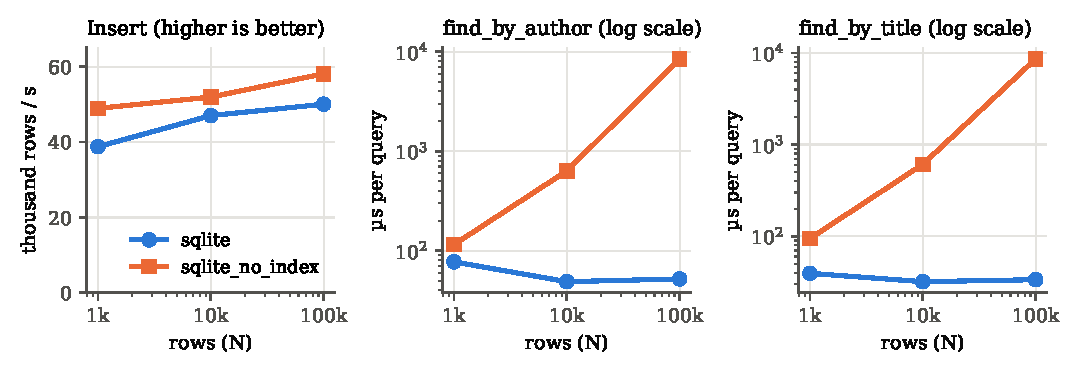
\includegraphics[width=\linewidth]{figures/metadata.pdf}
\caption{Insert throughput and average query cost as the table grows (logarithmic axes).}
\end{figure}

\begin{table}[H]
\centering\small
\begin{tabular}{@{}lrrr@{}}
\toprule
Metric (N = 100,000) & \code{sqlite} & \code{sqlite\_no\_index} & Ratio \\
\midrule
Insert (rows/s) & 50,036 & 58,103 & $\times$1.2 \\
\code{find\_by\_id} (\us) & 24.0 & 24.4 & $\times$1.0 \\
\code{find\_by\_author} (\us) & 52.0 & 8,459.6 & $\times$162.6 \\
\code{find\_by\_title} (\us) & 33.5 & 8,608.9 & $\times$256.8 \\
\bottomrule
\end{tabular}
\end{table}

\textbf{Discussion.}
\begin{itemize}
  \item \textbf{Queries by author or title:} without an index SQLite performs a full scan, so the
        cost grows linearly with N: from 115.1\us{} with 1,000 rows to 8,459.6\us{} with 100,000.
        With an index (a B-tree) it is logarithmic and almost flat: 77.2 $\rightarrow$ 52.0\us. With
        100,000 rows the index is about 160 times faster.
  \item \textbf{\code{find\_by\_id}} is the same in both variants, because both have the PRIMARY KEY
        (SQLite organises the table by \code{book\_id}). Its 24\us{} is essentially the fixed cost of
        one JDBC query: the floor for any query in this implementation.
  \item \textbf{Insertion:} maintaining two indexes has a price, since every new row also updates
        two B-trees, so the variant without indexes inserts faster. This is the classic trade-off:
        fast reads for slower writes and more disk.
  \item \textbf{Batching:} transactions of 1,000 rows are essential; with autocommit each row would
        be its own transaction with its own disk sync.
\end{itemize}

\subsection{Inverted-index benchmark}
Data: the 200 real books, with the SPEC tokenizer. Sizes: 50, 100 and 200 books (lowest ids first).
With 200 books the logical index has 129,356 terms and 1,581,064 postings (term--book pairs),
identical in the three backends. Each book contributes 7,905 distinct terms on average.

\textbf{Fairness rules:} all books are tokenized once before measuring (the tokenizer does not
pollute the times); before each repetition \code{freshIndex} clears the backend and checks that it
is empty; after measuring, \code{verify} compares the index with an in-memory one built from the same
terms. MongoDB uses its own database, \code{search\_engine\_bench}.

\begin{table}[H]
\centering\small
\begin{tabularx}{\linewidth}{@{}l Y l@{}}
\toprule
Experiment & What exactly is measured & Metrics \\
\midrule
\code{index\_build} & From an empty index to a persisted one: N \code{addDocument} with precomputed terms + one \code{flush}. Excludes reading, tokenizing, clearing and connecting. & elapsed, throughput \\
\code{index\_query} & The index is built and reopened; 100 runs of \code{queries.txt} through \code{SearchService} (query tokenization included). & elapsed, per\_query (\us) \\
\code{index\_update} & Index with N$-$k books (k = 10\%), reopened; adding the k books with one \code{flush} per book, as the \code{Indexer} does. & elapsed, per\_book (ms) \\
\code{index\_memory} & Java heap (after requesting GC) with the index built and freshly reopened. & heap\_after\_build/open \\
\code{index\_disk} & After building: logical bytes, files and allocated blocks. & bytes, files, terms, postings \\
\bottomrule
\end{tabularx}
\end{table}

\begin{figure}[H]
\centering
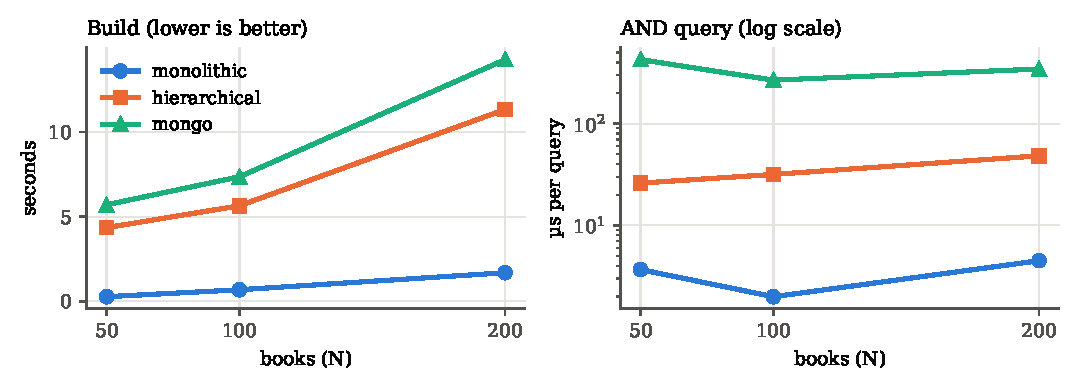
\includegraphics[width=\linewidth]{figures/index_build_query.pdf}
\caption{Build time and query cost against the number of books.}
\end{figure}

\begin{figure}[H]
\centering
\begin{minipage}[c]{0.55\linewidth}
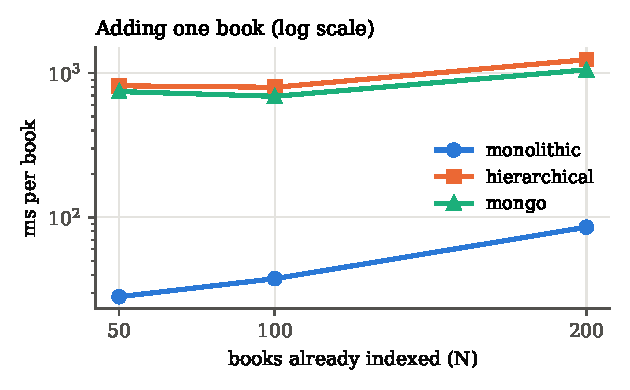
\includegraphics[width=\linewidth]{figures/index_update.pdf}
\end{minipage}\hfill
\begin{minipage}[c]{0.42\linewidth}\small
\caption{Cost of adding one book (log scale). Only \code{monolithic} grows with the index: its flush
rewrites the whole JSON. \code{hierarchical} and \code{mongo} only depend on the added book's terms
(about 0.1~ms per term in both).}
\end{minipage}
\end{figure}

\begin{figure}[H]
\centering
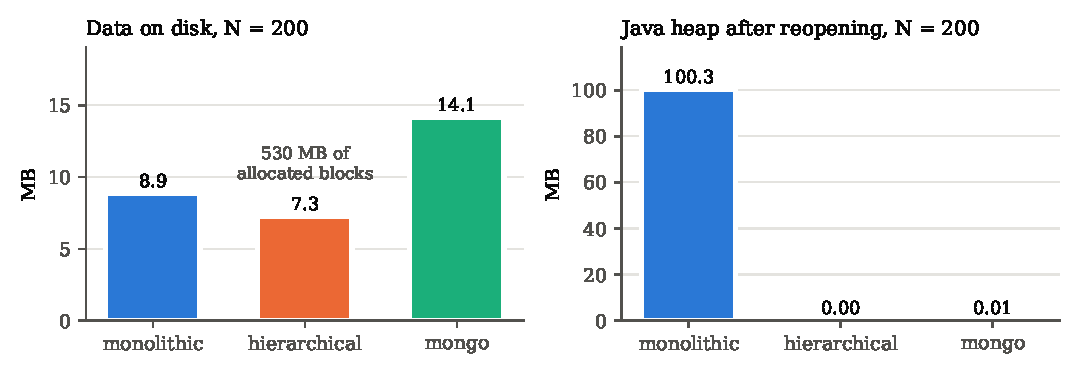
\includegraphics[width=\linewidth]{figures/index_disk_memory.pdf}
\caption{With 200 books: data on disk (left) and Java heap with the index freshly reopened (right).}
\end{figure}

\begin{table}[H]
\centering\small
\begin{tabular}{@{}lrrr@{}}
\toprule
Metric (median) & N = 50 & N = 100 & N = 200 \\
\midrule
Build (s) $\cdot$ monolithic & 0.27 & 0.68 & 1.69 \\
Build (s) $\cdot$ hierarchical & 4.35 & 5.65 & 11.34 \\
Build (s) $\cdot$ mongo & 5.70 & 7.36 & 14.29 \\
\midrule
Query (\us) $\cdot$ monolithic & 3.7 & 2.0 & 4.5 \\
Query (\us) $\cdot$ hierarchical & 26.0 & 31.7 & 48.3 \\
Query (\us) $\cdot$ mongo & 426.4 & 267.9 & 344.8 \\
\midrule
Update per book (ms) $\cdot$ monolithic & 28.1 & 37.5 & 85.4 \\
Update per book (ms) $\cdot$ hierarchical & 816.3 & 797.2 & 1,239.0 \\
Update per book (ms) $\cdot$ mongo & 744.5 & 690.0 & 1,052.7 \\
Average terms of the added books & 7,592 & 8,037 & 10,415 \\
\midrule
Disk (MB) $\cdot$ monolithic & 1.90 & 3.75 & 8.89 \\
Disk (MB) $\cdot$ hierarchical & 1.15 & 2.74 & 7.25 \\
Disk (MB) $\cdot$ mongo & 3.98 & 7.27 & 14.13 \\
Allocated blocks (MB) $\cdot$ hierarchical & 241.1 & 323.0 & 530.0 \\
Heap after reopening (MB) $\cdot$ monolithic & 18.50 & 48.29 & 100.33 \\
Heap after reopening (MB) $\cdot$ hierarchical & 0.00 & 0.00 & 0.00 \\
Heap after reopening (MB) $\cdot$ mongo & 0.01 & 0.02 & 0.01 \\
\midrule
Terms & 58,834 & 78,820 & 129,356 \\
Postings & 360,970 & 759,087 & 1,581,064 \\
\bottomrule
\end{tabular}
\end{table}

\textbf{Discussion.}
\begin{itemize}
  \item \textbf{Build:} \code{monolithic} is by far the fastest (1.69~s for 200 books): everything
        happens in memory and one file is written at the end. \code{hierarchical} (11.3~s) writes
        one file per term (129,356 files, each with its temp file and rename: about 88\us{} per
        file) and \code{mongo} (14.3~s) sends one upsert per term while the server maintains its
        unique index. \code{monolithic}'s throughput falls from 187 to 119 books/s as N grows: the
        \code{TreeMap} and the final JSON keep getting larger.
  \item \textbf{Queries:} \code{monolithic} answers in 4.5\us{} because the posting lists are
        already in memory; \code{hierarchical} reads one file per term and grows with N because each
        file holds more ids (26.0 $\rightarrow$ 48.3\us); \code{mongo} (268--426\us) is dominated by
        the round trip to the server for each term, which is why it shows no clear trend with N.
  \item \textbf{Updates, the key result:} \code{monolithic}'s flush rewrites the entire JSON, so
        its cost per book grows with the index: 28.1 $\rightarrow$ 37.5 $\rightarrow$ 85.4~ms, about
        10~ms per MB of JSON. \code{hierarchical} and \code{mongo} only touch the added book's terms,
        and their cost per term is almost constant (about 0.1~ms in both). Their rise at N = 200 is
        not caused by the index but by those 20 books being longer (10,415 terms on average against
        7,592--8,037).
  \item \textbf{When does \code{monolithic} stop paying off?} At these sizes it still wins by a
        factor of 12, but it is the only curve that grows with the index. At about 10~ms per MB it
        would reach \code{mongo}'s 1~s per book when the JSON is around 100~MB; with about 44~KB of
        JSON per book, that is roughly 2,000--2,500 books. This is an extrapolation, not a
        measurement.
  \item \textbf{Disk:} the data sizes are of the same order (7.3--14.1~MB). \code{mongo} takes the
        most (14.1~MB against 8.9~MB for \code{monolithic}): it counts its data plus its unique index
        on \code{term}. \code{hierarchical} allocates 530~MB of blocks for 7.3~MB of data
        ($\times$73): each of its 129,356 files takes at least one 4~KB block
        (129,356 $\times$ 4,096~B = 530~MB, exactly what was measured).
  \item \textbf{Memory:} \code{monolithic} keeps the whole index on the heap: 100~MB with 200 books
        for an 8.9~MB JSON (about 63 bytes per posting, since each id is an \code{Integer} inside a
        \code{TreeSet}). It grows linearly (about 0.5~MB per book), so the full Gutenberg catalogue
        (more than 70,000 books) would need tens of GB. \code{hierarchical} and \code{mongo} stay
        near zero after the flush: the data is on disk or in another process.
\end{itemize}

\textbf{Limits of the memory measurement.} \code{System.gc()} is a request, not an order, so the
value is an estimate with noise of a few KB. For \code{mongo}, only the client heap (driver,
connections, pending changes) is visible: the data lives in the \code{mongod} process with its own
WiredTiger cache, shared by all collections and sized by configuration, so it is not comparable with
the Java heap. After building, \code{hierarchical} and \code{mongo} leave 0.5--2.1~MB on the heap
even though their flush empties the pending map: \code{HashMap.clear()} keeps the internal table,
whose size is a power of two that depends on the number of terms (131,072 slots $\times$ 4~bytes =
524,288~bytes for 50 and 100 books; 524,288 slots $\times$ 4~bytes = 2,097,152~bytes for 200,
exactly the values measured).

\subsection{Real versus synthetic data}\label{sec:realsyn}
The same experiments with N = 200, on the synthetic data of the first version and on the 200 real
books.

\begin{table}[H]
\centering\small
\begin{tabular}{@{}lrrr@{}}
\toprule
Metric (N = 200) & Synthetic & Real & Real / synthetic \\
\midrule
Datalake: bytes stored & 61.5 MB & 129.0 MB & $\times$2.1 \\
Datalake: lookup $\cdot$ time & 143.3\us & 94.5\us & $\times$0.7 \\
Index: terms & 29,716 & 129,356 & $\times$4.4 \\
Index: postings & 423,261 & 1,581,064 & $\times$3.7 \\
Build $\cdot$ monolithic & 0.29 s & 1.69 s & $\times$5.9 \\
Build $\cdot$ hierarchical & 2.68 s & 11.34 s & $\times$4.2 \\
Build $\cdot$ mongo & 2.98 s & 14.29 s & $\times$4.8 \\
Update per book $\cdot$ monolithic & 17.2 ms & 85.4 ms & $\times$5.0 \\
Update per book $\cdot$ hierarchical & 272.4 ms & 1,239.0 ms & $\times$4.5 \\
Update per book $\cdot$ mongo & 191.7 ms & 1,052.7 ms & $\times$5.5 \\
Disk $\cdot$ monolithic & 2.74 MB & 8.89 MB & $\times$3.2 \\
Disk $\cdot$ mongo & 2.67 MB & 14.13 MB & $\times$5.3 \\
Allocated blocks $\cdot$ hierarchical & 121.8 MB & 530.0 MB & $\times$4.4 \\
Heap after reopening $\cdot$ monolithic & 28.71 MB & 100.33 MB & $\times$3.5 \\
Query $\cdot$ monolithic & 2.6\us & 4.5\us & $\times$1.7 \\
Query $\cdot$ hierarchical & 36.6\us & 48.3\us & $\times$1.3 \\
Query $\cdot$ mongo & 289.3\us & 344.8\us & $\times$1.2 \\
\bottomrule
\end{tabular}
\end{table}

\begin{itemize}
  \item \textbf{The conclusions hold.} In every index experiment the ranking between backends is the
        same, and in the datalake \code{time} is still the only layout with a slow lookup.
  \item \textbf{The magnitudes do not.} Building, updating, disk and memory cost 3 to 6 times more
        with real books. The synthetic generator limits the vocabulary to 30,000 words and each book
        to about 2,116 distinct terms, while a real book contributes about 7,905 (proper names,
        numbers, rare words) and the vocabulary keeps growing: 129,356 terms with 200 books.
  \item \textbf{Queries barely change} ($\times$1.2--1.7): a query only touches the posting lists of
        its few terms, so it depends much less on the total index size.
  \item \textbf{Only visible with real data:} the uneven spread of ids (\code{range} with 220
        entries in one folder), \code{mongo} using more disk than \code{monolithic}, and the update
        cost depending on which book is added.
  \item \textbf{Lesson:} synthetic data is good for comparing structures with each other; sizing a
        system (how much disk, RAM or time) needs real data.
\end{itemize}

\subsection{Summary: which structure to choose}
\begin{table}[H]
\centering\small
\begin{tabularx}{\linewidth}{@{}Y l l@{}}
\toprule
If the priority is\ldots & Datalake & Index \\
\midrule
Looking books up by id / showing results & \code{book} or \code{range} & --- \\
Processing in arrival order & \code{time} & --- \\
Small folders even when ids are concentrated & \code{time} & --- \\
Fastest queries, small index & --- & \code{monolithic} \\
Adding books continuously (incremental ingestion) & \code{range} & \code{hierarchical} or \code{mongo} \\
Index larger than RAM (beyond about 2,000 real books) & --- & \code{hierarchical} or \code{mongo} \\
Little disk space & any & \code{monolithic} \\
Several processes querying / scaling out & --- & \code{mongo} \\
\bottomrule
\end{tabularx}
\end{table}

% ================================================================ 8
\section{Conclusions and future improvements}

\subsection{Conclusions}
The Java implementation delivers the complete Stage~1 data layer: crawler, datalake, metadata and
inverted-index datamarts, AND search and a control layer that survives interruptions. All the
structures required by the SPEC are implemented behind interfaces and selected by configuration,
the 12 benchmark experiments are reproducible and written in the common format, and the 357 tests,
including the end-to-end test and the check against the sample dataset, show that the system is
correct and recoverable. The sample dataset and the offline mode let anyone verify it in seconds
without network.

The benchmarks show that no structure wins everywhere. The \code{monolithic} index is the best
choice at the scale of this stage, but its update cost and memory grow with the index, so a larger
collection will need \code{hierarchical} or, better, \code{mongo}, which also prepares the system
for several processes querying at once. For the datalake, \code{book} and \code{range} suit lookups
by id, while \code{time} suits processing in arrival order.

\subsection{Limitations and future improvements}
\begin{itemize}
  \item \textbf{Control files shared between structures.} Changing the datalake or index structure
        with existing data leaves books out of the new datalake or index, because the control layer
        already lists them as done. In practice, delete \code{data/} (or use another
        \code{data.dir}) when switching. A cleaner design, one control folder per combination of
        structures, would need a change to SPEC section 8 agreed by the group.
  \item \textbf{Small sizes} ($\le$ 200 real books): enough to see the trends and estimate when
        \code{monolithic} stops paying off (about 2,000--2,500 books), but that point is an
        extrapolation; it should be measured with thousands of books.
  \item \textbf{Prefixes by id.} Each N takes the lowest ids, not a random sample, as the SPEC
        requires for cross-language comparison. Low ids are older classics and the last books to
        enter are longer, which is why the update cost rises at N = 200.
  \item \textbf{One machine and one run per configuration.} The median of 5 runs resists isolated
        pauses but not variation between runs (visible in the \code{mongo} queries).
  \item \textbf{No ranking.} Search returns sorted ids without relevance, since no term frequencies
        are stored (a SPEC decision). Ranking belongs to the following stages.
\end{itemize}

\end{document}
